\documentclass{article}
\usepackage[margin=1in]{geometry}
\usepackage{amsmath,amsthm,amssymb}
\usepackage{bbm,enumerate,mathtools}
\usepackage{tikz,pgfplots}
\usepackage{chessboard}
\usepackage[hidelinks]{hyperref}
\usepackage{multicol} % Problem 35
\usepackage{xstring} % Difficulty command
\usetikzlibrary{shapes.geometric}

\newenvironment{question}{\begin{trivlist}\item[\textbf{Question.}]}{\end{trivlist}}
\newenvironment{note}{\begin{trivlist}\item[\textbf{Note.}]}{\end{trivlist}}
\newenvironment{references}{\begin{trivlist}\item[\textbf{References.}]}{\end{trivlist}}
\newenvironment{related}{\begin{trivlist}\item[\textbf{Related.}]\end{trivlist}\begin{enumerate}}{\end{enumerate}}

\newcommand\score[1]{
\pgfmathsetmacro\pgfxa{#1+1}
\tikzstyle{scorestars}=[
  star,
  star points=5,
  star point ratio=2.25,
  draw,
  inner sep=3pt,
  anchor=outer point 5
]
  \begin{tikzpicture}[baseline]
    \draw[opacity=0] (0,-0.5) rectangle (0,0.2); % Workaround for whitespace at the bottom.
    \foreach \i in {1,...,4} {
      \pgfmathparse{(\i<=#1?"yellow":"gray")}
      \edef\starcolor{\pgfmathresult}
      \draw (\i*4.5ex,0) node[name=star\i,scorestars,fill=\starcolor]  {};
    }
  \end{tikzpicture}
}

\newcommand{\difficulty}[1]{%
  \IfEqCase{#1}{%
      {1}{
        
\begin{tikzpicture}[scale=0.7, baseline=0.9mm]%
          \definecolor{slopegreen}{rgb}{0.0, 0.5, 0.0}%
          \fill[slopegreen] (0.5,0.5) circle (0.5);%
        \end{tikzpicture}%
      }%
      {2}{
        
\begin{tikzpicture}[scale=0.7, baseline=0.9mm]%
          \definecolor{slopeblue}{rgb}{0.0, 0.44, 1.00}
          \fill[slopeblue] (0,0) rectangle (1,1);%
        \end{tikzpicture}%
      }%
      {3}{
\begin{tikzpicture}[scale=0.7, baseline=0.9mm]\fill (0,0.5)--(0.5, 0)--(1,0.5)--(0.5,1)--cycle; \end{tikzpicture}}%
      {4}{
\begin{tikzpicture}[scale=0.7, baseline=0.9mm]\fill (0.25,0)--(0,0.5)--(0.25,1)--(0.5,0.5)--cycle; \fill (0.75,0)--(0.5,0.5)--(0.75,1)--(1,0.5)--cycle;\end{tikzpicture}}%
      % you can add more cases here as desired
  }[\PackageError{difficulty}{Undefined difficulty level: #1}{}]%
}%
\newcommand{\rating}[2]{\difficulty{#1}\\\score{#2}\\}


\begin{document}
\rating{3}{2}
This one is based on correspondence from Alec Jones: Consider all of the ways of partitioning the complete graph on $n$ vertices
into smaller complete graphs.
\begin{figure}[!h]
  \centering
  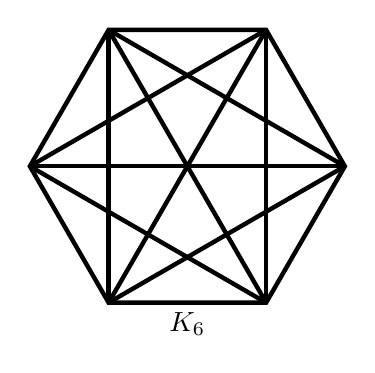
\begin{tikzpicture}[scale = 2]
    \draw[ultra thick] (-1,0)
      --(-0.5,{sqrt(3)/2})
      --(0.5,{sqrt(3)/2})
      --(1,0)
      --(0.5,{-sqrt(3)/2})
      --(-0.5,{-sqrt(3)/2})
      --cycle;

    \draw[ultra thick] (-1,0)--(0.5,{sqrt(3)/2});
    \draw[ultra thick] (-1,0)--(1,0);
    \draw[ultra thick] (-1,0)--(0.5,{-sqrt(3)/2});

    \draw[ultra thick] (-0.5,{sqrt(3)/2})--(1,0);
    \draw[ultra thick] (-0.5,{sqrt(3)/2})--(0.5,{-sqrt(3)/2});
    \draw[ultra thick] (-0.5,{sqrt(3)/2})--(-0.5,{-sqrt(3)/2});

    \draw[ultra thick] (0.5,{sqrt(3)/2})--(0.5,{-sqrt(3)/2});
    \draw[ultra thick] (0.5,{sqrt(3)/2})--(-0.5,{-sqrt(3)/2});

    \draw[ultra thick] (1,0)--(-0.5,{-sqrt(3)/2});
    \node at (0, -1) { $K_6$ };
  \end{tikzpicture}
  \\~\\
  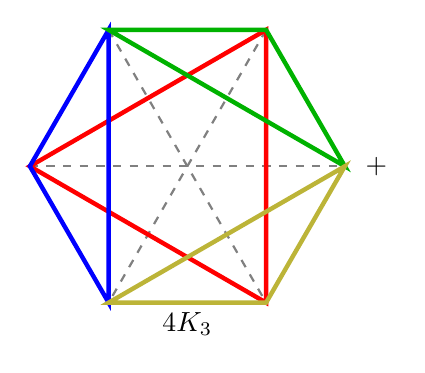
\begin{tikzpicture}[scale = 2]
    \draw[gray,thick,dashed] (-1,0)
      --(-0.5,{sqrt(3)/2})
      --(0.5,{sqrt(3)/2})
      --(1,0)
      --(0.5,{-sqrt(3)/2})
      --(-0.5,{-sqrt(3)/2})
      --cycle;
    \draw[gray,thick,dashed] (-1,0)--(0.5,{sqrt(3)/2});
    \draw[gray,thick,dashed] (-1,0)--(1,0);
    \draw[gray,thick,dashed] (-1,0)--(0.5,{-sqrt(3)/2});
    \draw[gray,thick,dashed] (-0.5,{sqrt(3)/2})--(1,0);
    \draw[gray,thick,dashed] (-0.5,{sqrt(3)/2})--(0.5,{-sqrt(3)/2});
    \draw[gray,thick,dashed] (-0.5,{sqrt(3)/2})--(-0.5,{-sqrt(3)/2});
    \draw[gray,thick,dashed] (0.5,{sqrt(3)/2})--(0.5,{-sqrt(3)/2});
    \draw[gray,thick,dashed] (0.5,{sqrt(3)/2})--(-0.5,{-sqrt(3)/2});
    \draw[gray,thick,dashed] (1,0)--(-0.5,{-sqrt(3)/2});

    \draw[red,ultra thick] (-1,0)
      --(0.5,{sqrt(3)/2})
      --(0.5,{-sqrt(3)/2})
      --cycle;
    \draw[blue,ultra thick] (-1,0)
      --(-0.5,{sqrt(3)/2})
      --(-0.5,{-sqrt(3)/2})
      --cycle;
    \draw[black!30!green,ultra thick] (1,0)
      --(-0.5,{sqrt(3)/2})
      --(0.5,{sqrt(3)/2})
      --cycle;
    \draw[black!30!yellow,ultra thick] (1,0)
      --(-0.5,{-sqrt(3)/2})
      --(0.5,{-sqrt(3)/2})
      --cycle;
    \node at (0, -1) { $4K_3$ };
    \node at (1.2, 0) {$+$};
  \end{tikzpicture}
  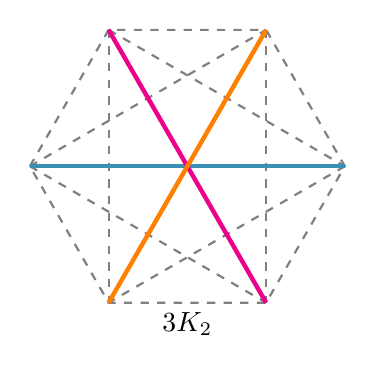
\begin{tikzpicture}[scale = 2]
    \draw[gray,thick,dashed] (-1,0)
      --(-0.5,{sqrt(3)/2})
      --(0.5,{sqrt(3)/2})
      --(1,0)
      --(0.5,{-sqrt(3)/2})
      --(-0.5,{-sqrt(3)/2})
      --cycle;
    \draw[gray,thick,dashed] (-1,0)--(0.5,{sqrt(3)/2});
    \draw[gray,thick,dashed] (-1,0)--(1,0);
    \draw[gray,thick,dashed] (-1,0)--(0.5,{-sqrt(3)/2});
    \draw[gray,thick,dashed] (-0.5,{sqrt(3)/2})--(1,0);
    \draw[gray,thick,dashed] (-0.5,{sqrt(3)/2})--(0.5,{-sqrt(3)/2});
    \draw[gray,thick,dashed] (-0.5,{sqrt(3)/2})--(-0.5,{-sqrt(3)/2});
    \draw[gray,thick,dashed] (0.5,{sqrt(3)/2})--(0.5,{-sqrt(3)/2});
    \draw[gray,thick,dashed] (0.5,{sqrt(3)/2})--(-0.5,{-sqrt(3)/2});
    \draw[gray,thick,dashed] (1,0)--(-0.5,{-sqrt(3)/2});

    \draw[black!30!cyan,ultra thick] (-1,0)--(1,0);
    \draw[magenta,ultra thick] (-0.5,{sqrt(3)/2})--(0.5,{-sqrt(3)/2});
    \draw[orange,ultra thick] (0.5,{sqrt(3)/2})--(-0.5,{-sqrt(3)/2});
    \node at (0, -1) { $3K_2$ };
  \end{tikzpicture}
  \\~\\
  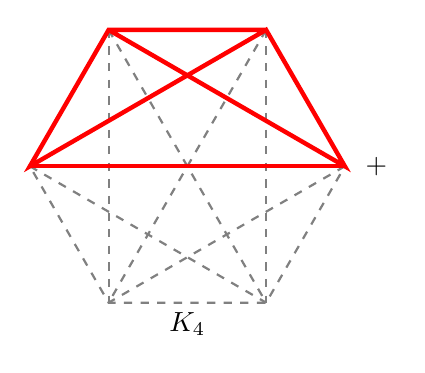
\begin{tikzpicture}[scale = 2]
    \draw[gray,thick,dashed] (-1,0)
      --(-0.5,{sqrt(3)/2})
      --(0.5,{sqrt(3)/2})
      --(1,0)
      --(0.5,{-sqrt(3)/2})
      --(-0.5,{-sqrt(3)/2})
      --cycle;
    \draw[gray,thick,dashed] (-1,0)--(0.5,{sqrt(3)/2});
    \draw[gray,thick,dashed] (-1,0)--(1,0);
    \draw[gray,thick,dashed] (-1,0)--(0.5,{-sqrt(3)/2});
    \draw[gray,thick,dashed] (-0.5,{sqrt(3)/2})--(1,0);
    \draw[gray,thick,dashed] (-0.5,{sqrt(3)/2})--(0.5,{-sqrt(3)/2});
    \draw[gray,thick,dashed] (-0.5,{sqrt(3)/2})--(-0.5,{-sqrt(3)/2});
    \draw[gray,thick,dashed] (0.5,{sqrt(3)/2})--(0.5,{-sqrt(3)/2});
    \draw[gray,thick,dashed] (0.5,{sqrt(3)/2})--(-0.5,{-sqrt(3)/2});
    \draw[gray,thick,dashed] (1,0)--(-0.5,{-sqrt(3)/2});

    \draw[red,ultra thick] (-0.5,{sqrt(3)/2})
      --(1,0)
      --(0.5,{sqrt(3)/2})
      --(-1,0)
      --(-0.5,{sqrt(3)/2})
      --(0.5,{sqrt(3)/2});
    \draw[red,ultra thick](1,0)--(-1,0);
    \node at (0, -1) { $K_4$ };
    \node at (1.2, 0) {$+$};
  \end{tikzpicture}
  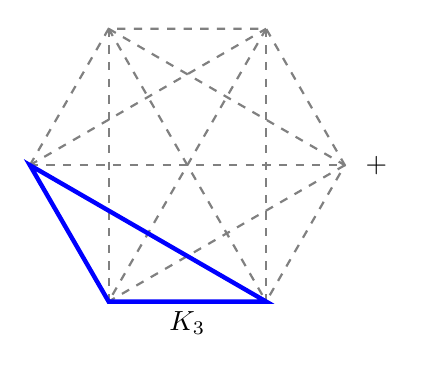
\begin{tikzpicture}[scale = 2]
    \draw[gray,thick,dashed] (-1,0)
      --(-0.5,{sqrt(3)/2})
      --(0.5,{sqrt(3)/2})
      --(1,0)
      --(0.5,{-sqrt(3)/2})
      --(-0.5,{-sqrt(3)/2})
      --cycle;
    \draw[gray,thick,dashed] (-1,0)--(0.5,{sqrt(3)/2});
    \draw[gray,thick,dashed] (-1,0)--(1,0);
    \draw[gray,thick,dashed] (-1,0)--(0.5,{-sqrt(3)/2});
    \draw[gray,thick,dashed] (-0.5,{sqrt(3)/2})--(1,0);
    \draw[gray,thick,dashed] (-0.5,{sqrt(3)/2})--(0.5,{-sqrt(3)/2});
    \draw[gray,thick,dashed] (-0.5,{sqrt(3)/2})--(-0.5,{-sqrt(3)/2});
    \draw[gray,thick,dashed] (0.5,{sqrt(3)/2})--(0.5,{-sqrt(3)/2});
    \draw[gray,thick,dashed] (0.5,{sqrt(3)/2})--(-0.5,{-sqrt(3)/2});
    \draw[gray,thick,dashed] (1,0)--(-0.5,{-sqrt(3)/2});

    \draw[blue,ultra thick] (-0.5,{-sqrt(3)/2})
      --(0.5,{-sqrt(3)/2})
      --(-1,0)
      --cycle;
    \node at (0, -1) { $K_3$ };
    \node at (1.2, 0) {$+$};
  \end{tikzpicture}
  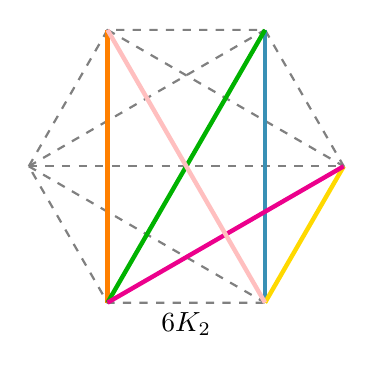
\begin{tikzpicture}[scale = 2]
    \draw[gray,thick,dashed] (-1,0)
      --(-0.5,{sqrt(3)/2})
      --(0.5,{sqrt(3)/2})
      --(1,0)
      --(0.5,{-sqrt(3)/2})
      --(-0.5,{-sqrt(3)/2})
      --cycle;
      \draw[gray,thick,dashed] (-1,0)--(0.5,{sqrt(3)/2});
      \draw[gray,thick,dashed] (-1,0)--(1,0);
      \draw[gray,thick,dashed] (-1,0)--(0.5,{-sqrt(3)/2});
      \draw[gray,thick,dashed] (-0.5,{sqrt(3)/2})--(1,0);
      \draw[gray,thick,dashed] (-0.5,{sqrt(3)/2})--(0.5,{-sqrt(3)/2});
      \draw[gray,thick,dashed] (-0.5,{sqrt(3)/2})--(-0.5,{-sqrt(3)/2});
      \draw[gray,thick,dashed] (0.5,{sqrt(3)/2})--(0.5,{-sqrt(3)/2});
      \draw[gray,thick,dashed] (0.5,{sqrt(3)/2})--(-0.5,{-sqrt(3)/2});
      \draw[gray,thick,dashed] (1,0)--(-0.5,{-sqrt(3)/2});

      \draw[black!30!cyan,ultra thick] (0.5,{sqrt(3)/2})--(0.5,{-sqrt(3)/2});
      \draw[orange!30!yellow,ultra thick] (1,0)--(0.5,{-sqrt(3)/2});
      \draw[orange,ultra thick] (-0.5,{sqrt(3)/2})--(-0.5,{-sqrt(3)/2});
      \draw[black!30!green,ultra thick] (0.5,{sqrt(3)/2})--(-0.5,{-sqrt(3)/2});
      \draw[magenta,ultra thick] (1,0)--(-0.5,{-sqrt(3)/2});
      \draw[pink, ultra thick] (-0.5,{sqrt(3)/2})--(0.5,{-sqrt(3)/2});
      \node at (0, -1) { $6K_2$ };
  \end{tikzpicture}

  \caption{
    An example three ways to partition $K_6$ into complete graphs: the trivial
    partition, a partition into $4$ copies of $K_3$ and $3$ copies of $K_2$, and
    a partition into $1$ copy of $K_4$, $1$ copy of $K_3$, and $6$ copies of $K_2$.
  }
\end{figure}

\begin{question}
  How many such partitions exist, up to graph isomorphism?
\end{question}
\begin{related}
  \item What if the union of $K_j$ graphs cannot contain a $K_{j-1}$ subgraph?
  \item What if the partition can only consist of two ``sizes'' of complete
    graphs, as in the second example?
  \item How many such partitions exist up to dihedral action?
\end{related}
\end{document}
